\section{RESULTS}
% Edit below
Tussentitels per topic/techniek (4.1, 4.1.1, \dots).
Beschrijf de resultaten (interpreteer ze nog niet), wat zie je (objectief)?
Zorg dat figuren een caption hebben (incl. alle afkortingen) onder de figuur en dat je zeker in de tekst refereert naar desbetreffende figuur. 
Tabellen krijgen een caption bovenaan (zelfde principe).

Willen jullie resultaten tonen zoals figuren dan dienen jullie de \textit{figure} environment gebruiken.
\textbf{LET OP}: in deze template dient de figure environment altijd met de 'H' parameter gebruikt te worden.
\begin{figure}[H]
    \centering
    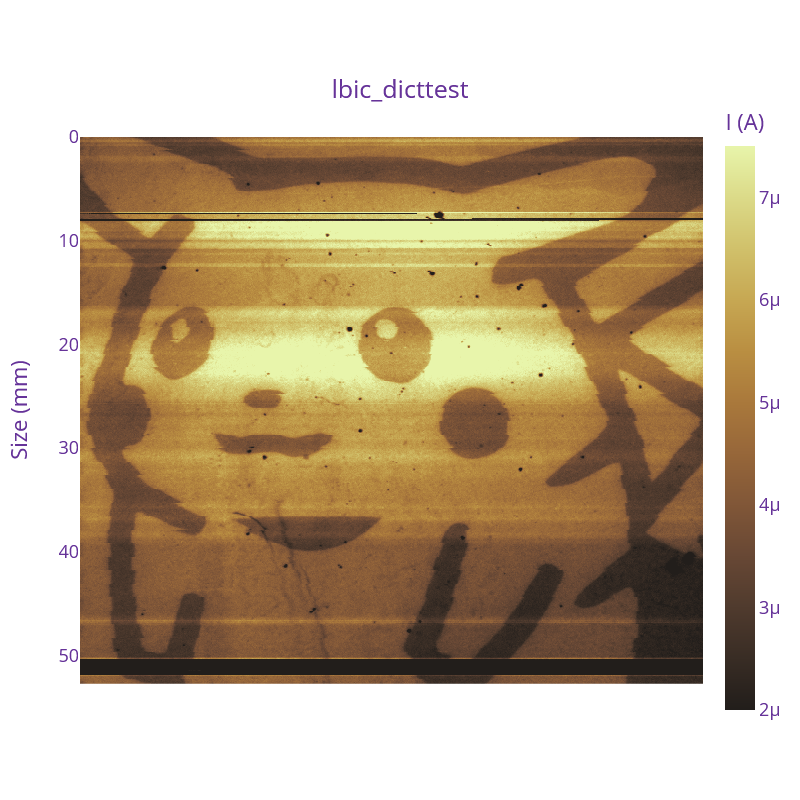
\includegraphics[width=\linewidth]{Figures/newplot(4).png}
    \caption{Dit is het onderschrift van deze figuur}
    \label{fig:pikachu}
\end{figure}

Tabellen moeten in de \textit{table} environment geplaatst worden.
Ook hier is de 'H' parameter cruciaal.
Gebruik \url{https://www.tablesgenerator.com/} voor hulp bij de opmaak van tabellen.
\begin{table}[H]
\centering
 \begin{tabular}{||c c c c||} 
 \hline
 Col1 & Col2 & Col2 & Col3 \\ [0.5ex] 
 \hline\hline
 1 & 6 & 87837 & 787 \\ 
 2 & 7 & 78 & 5415 \\
 3 & 545 & 778 & 7507 \\
 4 & 545 & 18744 & 7560 \\
 5 & 88 & 788 & 6344 \\ [1ex] 
 \hline
 \end{tabular}
\end{table}